\documentclass[12pt]{jarticle}
\usepackage{TUSIReport}
\usepackage{otf}
\usepackage[dvipdfmx]{graphicx}
\usepackage[dvipdfmx]{color}
\usepackage{amsmath}
\usepackage{amssymb}
\usepackage{color}
\usepackage{hhline}
\usepackage{fancybox,ascmac}
\usepackage{multirow}
\usepackage{url}
\usepackage{bm}
\usepackage{listings,jlisting}
\lstdefinestyle{log}{
    frame={tblr},
    basicstyle={\footnotesize},
    tabsize={4},
}
\lstdefinestyle{lstcpp}{
    language={c++},
    backgroundcolor={\color[gray]{.85}},
    basicstyle={\small},
    identifierstyle={\small},
    commentstyle={\small\ttfamily \color[rgb]{0,0.5,0}},
    keywordstyle={\small\bfseries \color[rgb]{1,0,0}},
    ndkeywordstyle={\small},
    stringstyle={\small\ttfamily \color[rgb]{0,0,1}},
    frame={tb},
    breaklines=true,
    columns=[l]{fullflexible},
    numbers=left,
    xrightmargin=0zw,
    xleftmargin=3zw,
    numberstyle={\scriptsize},
    stepnumber=1,
    numbersep=1zw,
    morecomment=[l]{//}
}
\begin{document}
%%%%%%%%%%%%%%%%%%%%%%%%%%%%%%%%%%%%%%%%%%%%%%%%%%%%%%%%%%%%%%
% 表紙を出力する場合は,\提出者と\共同実験者をいれる
% \提出者{科目名}{課題名}{提出年}{提出月}{提出日}{学籍番号}{氏名}
% \共同実験者{一人目}{二人目}{..}{..}{..}{..}{..}{八人目}
%%%%%%%%%%%%%%%%%%%%%%%%%%%%%%%%%%%%%%%%%%%%%%%%%%%%%%%%%%%%%%
\提出者{情報工学実験2}{実験テーマ3 情報通信シミュレーション}{2020}{11}{30}{4619055}{辰川力駆}
\共同実験者{}{}{}{}{}{}{}{}

%%%%%%%%%%%%%%%%%%%%%%%%%%%%%%%%%%%%%%%%%%%%%%%%%%%%%%%%%%%%%%
% 表紙を出力しない場合は,以下の「\表紙出力」をコメントアウトする
%%%%%%%%%%%%%%%%%%%%%%%%%%%%%%%%%%%%%%%%%%%%%%%%%%%%%%%%%%%%%%
\表紙出力

%%%%%%%%%%%%%%%%%%%%%%%%%%%%%%%%%%%%%%%%%%%%%%%%%%%%%%%%%%%%%%
% 以下はレポート本体である.別途 TeXファイルを作成し \input 使っても良い
%%%%%%%%%%%%%%%%%%%%%%%%%%%%%%%%%%%%%%%%%%%%%%%%%%%%%%%%%%%%%%

\section{実験概要}
rand() によって発生させた乱数と、MT によって発生させた乱数それぞれに
ついて誤り率をプロットしたグラフを作成するなどをして、
ディジタル通信システムと誤り訂正符号の理解を深める。

\section{実験手順}
\begin{itemize}
    \item 系列長$K=4$の情報系列
          $w=(w_1,...,w_K) \in \{0,1\}$ を乱数によって
          発生させ、
          BSCの各$\epsilon$に対するビット誤り率の値をシミュレーション
          により求める。
          乱数の発生には、C 言語コンパイラ上で rand() 関数を用いたものと
          Mersenne Twister (MT) を用いた 2 種類のプログラムを作成する。
    \item 横軸を BSC の誤り確率 $\epsilon$、縦軸 (指数表示) を
          ビット誤り率 $P_e$ としてグラフにプロットする。
    \item 誤り確率の理論値 ($\epsilon$) を実線 (プロットなし) で表示してシミュレー
          ションで得られた値と比較する。
\end{itemize}

\section{実験結果}
\begin{lstlisting}[style=log,caption=rand()関数の結果(ep0.0001)]
    # SIM:1000000
    # ep   # BER
    0.0001 0.0001060
    0.0002 0.0001970
    0.0003 0.0002992
    0.0004 0.0004087
    0.0005 0.0004960
    0.0006 0.0006067
    0.0007 0.0007080
    0.0008 0.0008005
    0.0009 0.0008992
    0.0010 0.0010153
    0.0011 0.0010995
    0.0012 0.0012267
\end{lstlisting}

\clearpage
\begin{lstlisting}[style=log,caption=MTの結果(ep0.0001)]
    # SIM:1000000
    # ep   # BER
    0.0001 0.0001033
    0.0002 0.0002025
    0.0003 0.0002958
    0.0004 0.0003975
    0.0005 0.0004955
    0.0006 0.0005958
    0.0007 0.0007170
    0.0008 0.0008185
    0.0009 0.0008900
    0.0010 0.0009938
    0.0011 0.0010995
    0.0012 0.0012400
\end{lstlisting}

ソースコードは付録に記述した。
$\epsilon=0.0001$として、SIMを1000000回実行した結果は上記のようになった。
また、それらの結果をグラフにプロットすると図1のようになった。
なお、縦軸は対数で表示している。

\begin{figure}[h]
    \begin{center}
        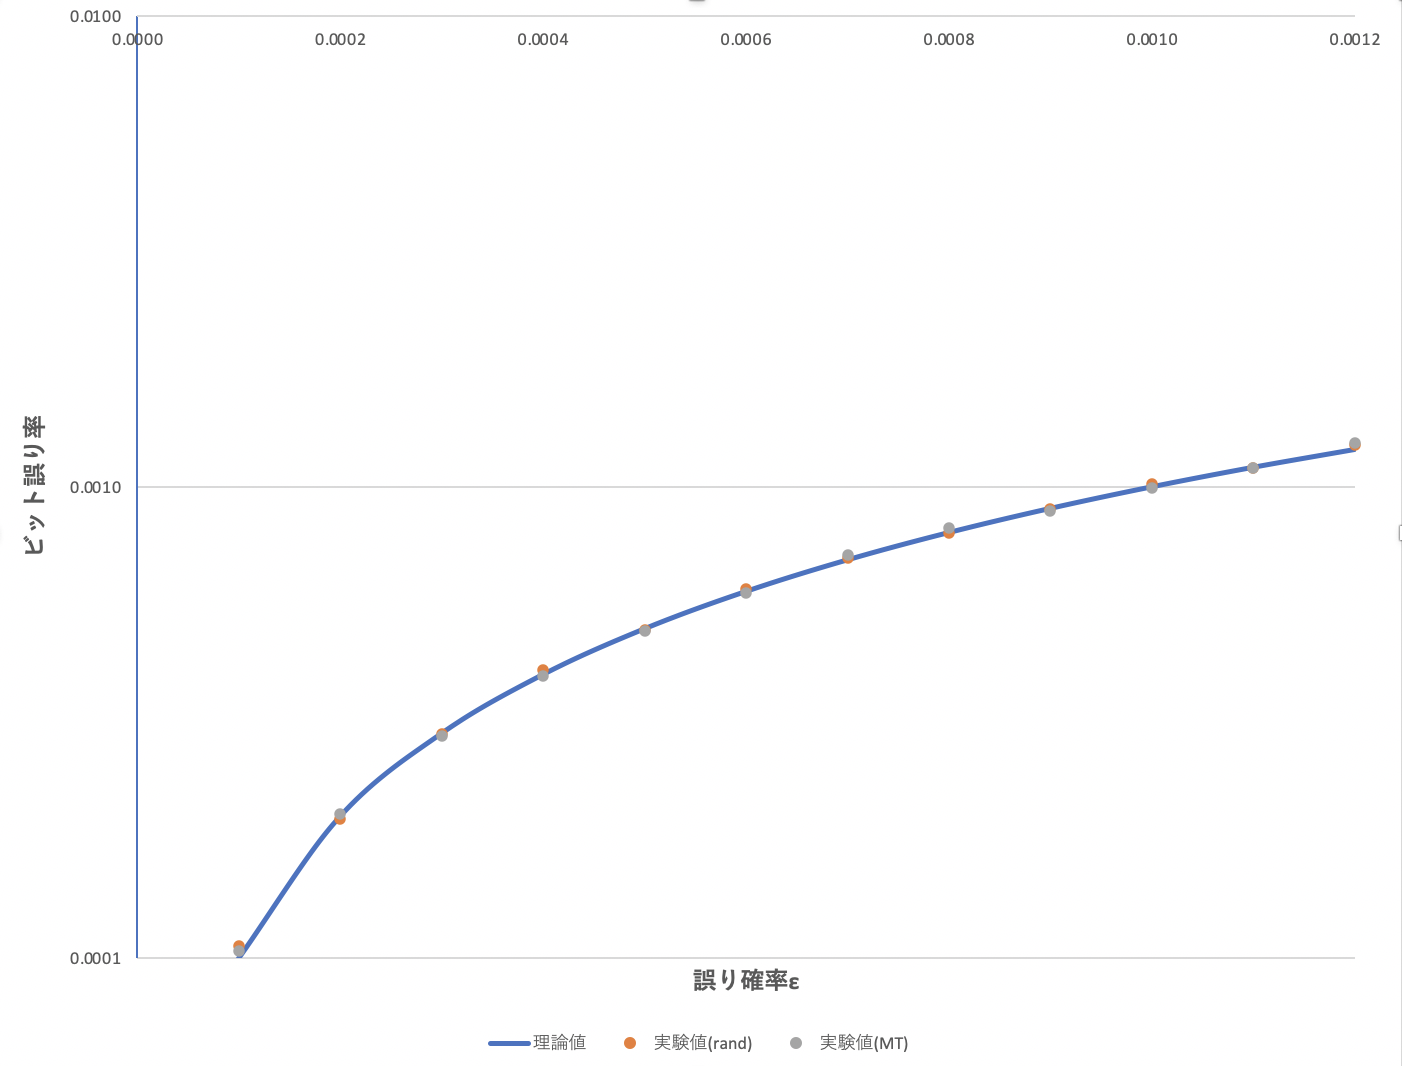
\includegraphics[scale=0.3]{kadai3_1_1.png}
    \end{center}
    \caption{ビット誤り率と誤り確率}
\end{figure}

\section{検討}
\subsection{課題1}
\begin{shadebox}
    シミュレーションによるビット誤り率と理論値が
    ほぼ同じ値になるにはどの程度のシミュレーション回数を実行する必要があるか。
\end{shadebox}

大数の法則より、シミュレーション回数を増やすほうが、
理論値に近づくのは明白である。
実際、SIM回数を1000000回から減らすと、
誤差が大きくなった。
さらに誤差を減らすためには1000000回以上行えばよいが、
実行するのに時間とてもかかってしまうだろう。

\subsection{課題2}
\begin{shadebox}
    $\epsilon$を非常に小さくした場合、これはどうなるか。
\end{shadebox}

$\epsilon$を実験よりさらに10分の1の値($\epsilon=0.00001$)とした場合、
以下のような結果となった。
行うことは同様であったが、誤差の割合を見ると大きくなっていると考えられる。
これは、理論値を小さくすることにより相対的に誤差の割合が大きくなっていると考えられる。

\begin{lstlisting}[style=log,caption=rand()関数の結果(ep0.00001)]
    # SIM:1000000
    # ep   # BER
    0.00001 0.00001275
    0.00002 0.00001700
    0.00003 0.00003625
    0.00004 0.00004150
    0.00005 0.00004625
    0.00006 0.00006750
    0.00007 0.00007475
    0.00008 0.00008100
    0.00009 0.00008850
    0.00010 0.00010400
    0.00011 0.00011375
    0.00012 0.00012900
\end{lstlisting}

\begin{lstlisting}[style=log,caption=MTの結果(ep0.00001)]
    # SIM:1000000
    # ep   # BER
    0.00001 0.00000925
    0.00002 0.00002075
    0.00003 0.00002725
    0.00004 0.00003825
    0.00005 0.00004825
    0.00006 0.00006275
    0.00007 0.00007150
    0.00008 0.00008175
    0.00009 0.00009050
    0.00010 0.00009925
    0.00011 0.00011375
    0.00012 0.00012075    
\end{lstlisting}

\clearpage

\subsection{課題3}
\begin{shadebox}
    $\rm{rand()}$と$\rm{MT}$の違いは何か。
\end{shadebox}

rand()関数は環境にもよるが$0\sim 32767$までの値しか取らない。
環境が違っていても少なくとも最大値が存在する。
今回は$0\sim 1$の値を求めるだけに使ったのであまり変わらなかったが、
$0\sim 10000$の値を求めるために乱数を使ったりするときは、
最大値が存在するから偏りが生じる。
よって、ほぼ均等に乱数を生成するならばメルセンヌ・ツイスタを用いるほうが良いと考える。

しかし、メルセンヌ・ツイスタで実行した場合、
実行速度が(rand()関数を用いた時より)遅くなるので、
速度を重視するか、性能を重視するかで使い分けると良いだろう。

\clearpage
% 付録
\appendix
\section{付録}
\begin{lstlisting}[style = lstcpp,caption=kadai3\_rand.cpp]
    //4619055 辰川力駆
    #include <random> // 乱数生成
    #include <stdio.h>
    #include <iostream>
    #include <iomanip>
    
    using namespace std;
    
    #define SIM 1000000
    
    #define real_rand (double)rand() / RAND_MAX; //RAND_MAXで割ることで0から1を返すようにしている。
    #define seed 55                              //学籍番号下2桁
    #define K 4                                  //系列長
    
    int main()
    {
        srand(seed);
        int w[4], e[4], y[4];
    
        cout << "# SIM:" << SIM << endl;
        cout << "# ep   # BER" << endl;
    
        double ep = 0;
        int count = 0;
        for (int i = 0; i < 12; i++) //12回で設定
        {
            count = 0;
            ep = 0.0001 * (i + 1);
    
            for (int s = 0; s < SIM; s++)
            {
                for (int j = 0; j < K; j++)
                {
                    double rd = real_rand; //乱数発生
                    w[j] = rd * 2;         //2倍することで0.5より大きいか小さいかを判定できる。
                }
                for (int j = 0; j < K; j++)
                {
                    double rd = real_rand; //乱数発生
                    if (rd <= ep)
                    {
                        e[j] = 1;
                    }
                    else
                    {
                        e[j] = 0;
                    }
                }
                for (int j = 0; j < K; j++)
                {
                    y[j] = w[j] ^ e[j];
                    count += w[j] ^ y[j];
                }
            }
            cout << fixed << setprecision(4) << ep;
            cout.unsetf(ios::fixed);
            cout << fixed << setprecision(7) << " " << (double)count / (K * SIM) << endl;
        }
    
        return 0;
    }
\end{lstlisting}

\begin{lstlisting}[style = lstcpp,caption=kadai3\_mt.cpp]
    //4619055 辰川力駆
    #include <random> // 乱数生成
    #include <stdio.h>
    #include <iostream>
    #include <iomanip>
    
    using namespace std;
    
    #define SIM 1000000
    
    #define seed 55 //学籍番号下2桁
    #define K 4     //系列長
    
    mt19937 mt(seed); //メルセンヌ・ツイスタ
    
    int main()
    {
        srand(seed);
        int w[4], e[4], y[4];
    
        uniform_real_distribution<double> rand_real(0, 1);
        normal_distribution<double> rand_n(0, 0.3);
    
        cout << "# SIM:" << SIM << endl;
        cout << "# ep   # BER" << endl;
    
        double ep = 0;
        int count = 0;
        for (int i = 0; i < 12; i++) //12回で設定
        {
            count = 0;
            ep = 0.0001 * (i + 1);
    
            for (int s = 0; s < SIM; s++)
            {
                for (int j = 0; j < K; j++)
                {
                    w[j] = rand_real(mt) * 2; //2倍することで0.5より大きいか小さいかを判定できる。
                }
                for (int j = 0; j < K; j++)
                {
                    if (rand_real(mt) <= ep)
                    {
                        e[j] = 1;
                    }
                    else
                    {
                        e[j] = 0;
                    }
                }
                for (int j = 0; j < K; j++)
                {
                    y[j] = w[j] ^ e[j];
                    count += w[j] ^ y[j];
                }
            }
            cout << fixed << setprecision(4) << ep;
            cout.unsetf(ios::fixed);
            cout << fixed << setprecision(7) << " " << (double)count / (K * SIM) << endl;
        }
    
        return 0;
    }
\end{lstlisting}

%%%%%%%%%%%%%%%%%%%%%%%%%%%%%%%%%%%%%%%%%%%%%%%%%%%%%%%%%%%%%%
\end{document}